\section{Introduction}
\label{integriscreen:sec:intro}

In the previous chapter (Chapter \ref{ch:integrikey}), we describe \integrikey that provides a second factor for the integrity of the user input coming from a keyboard. However, this integrity guarantee is purely limited the keyboard input and does not take into account what the user sees on the screen. In other words, \integrikey is oblivious to the user's \emph{intent}. We use the term intent to establish the connection between what the user sees on display and what the user is typing in response to that. Similar to \integrikey, we assume an attacker that controls the software stack, that includes the OS and hypervisor of the host that the user has. A large class of web-based services and applications (e.g., online banking or remote database access) uses modern user interfaces (UIs) displayed on the browser to interact with the user. In all of these UIs, the user's intended input is displayed on the host's screen. Despite what a compromised host might attempt to do in the background, users communicate their intention by entering and modifying the values shown on the screen until they are satisfied with what they see or abort if they are prevented from doing so.


\begin{figure}[t]
 \centering
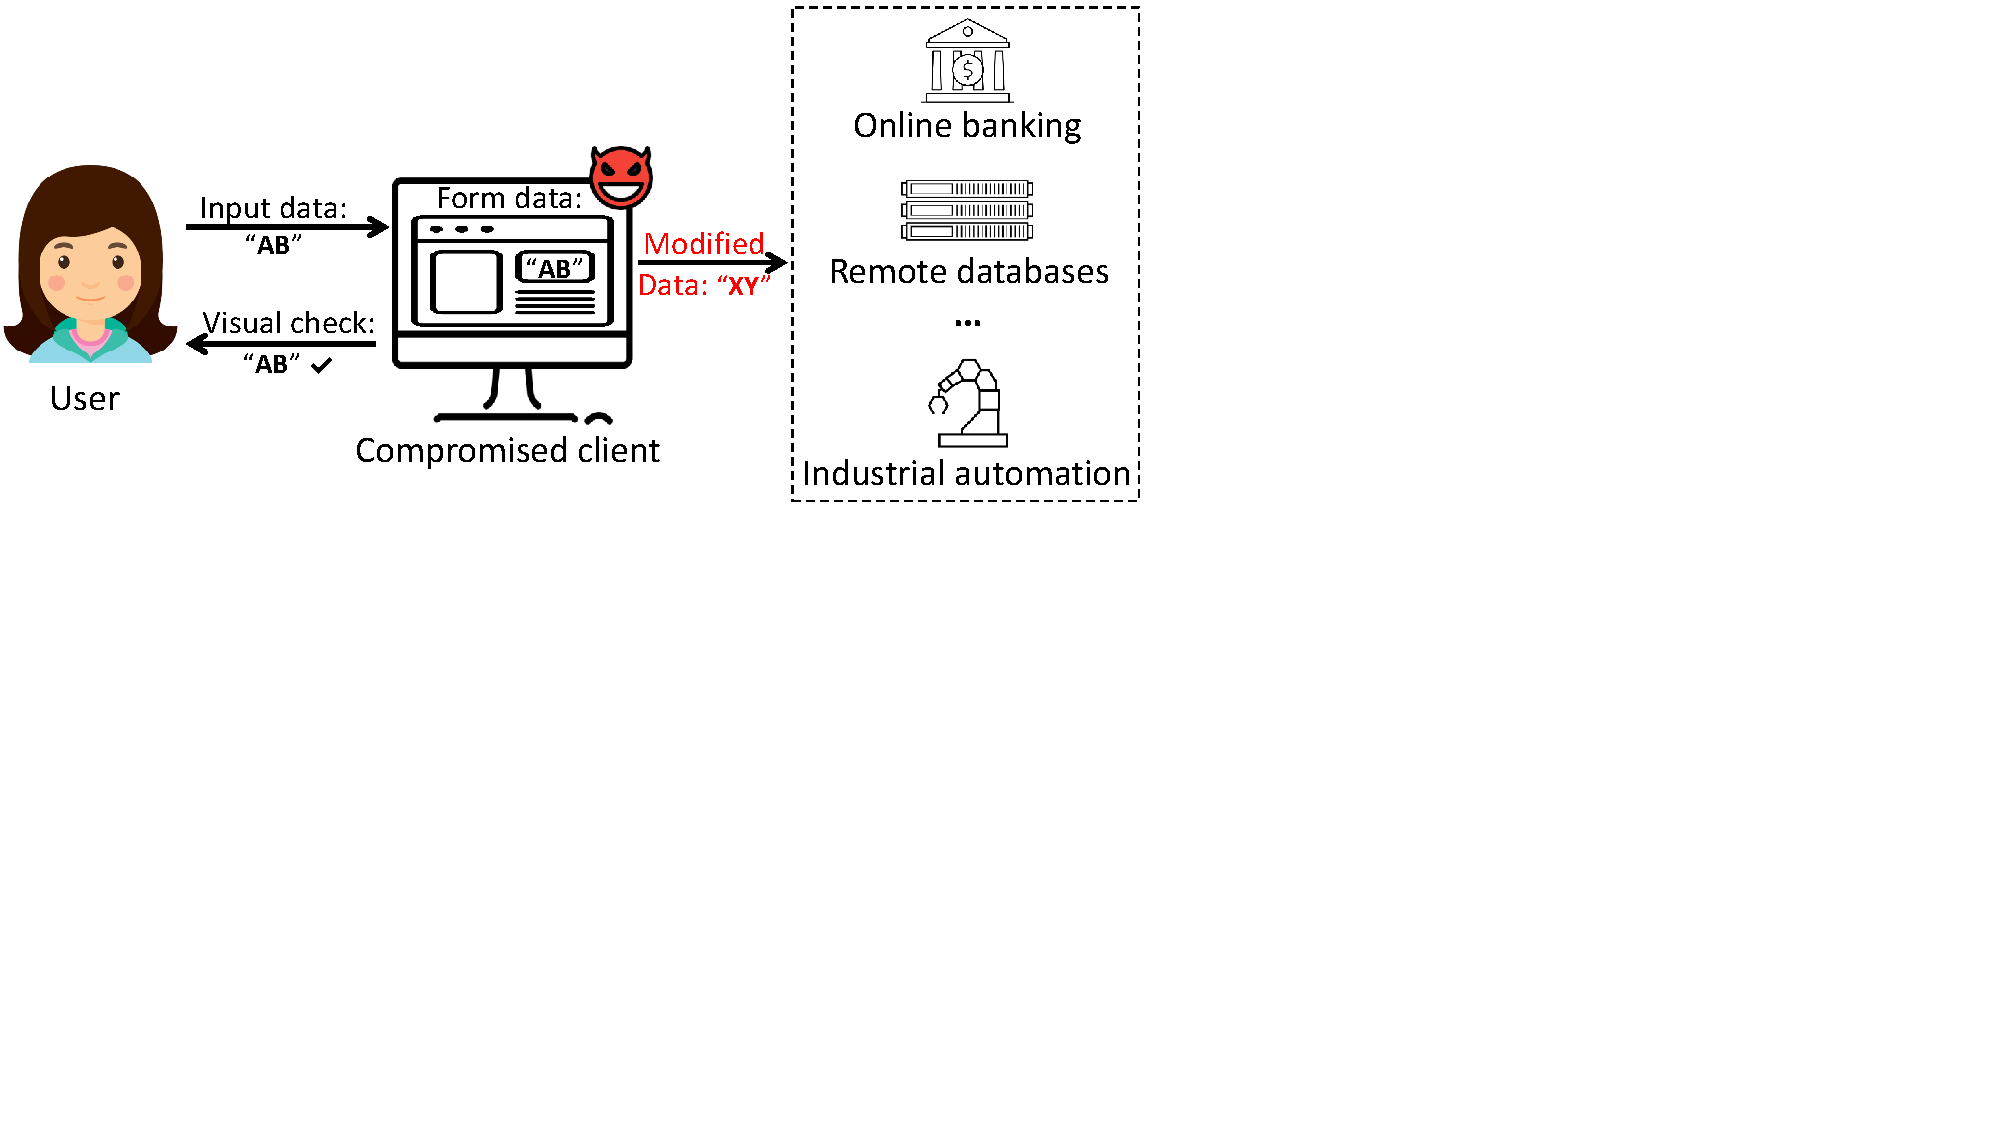
\includegraphics[trim={0 10.4cm 14.4cm 0},clip,width=0.75\linewidth]{chapters/IntegriScreen/img/motivatingScenario.pdf}
\caption[Attack scenario in a compromised host]{\textbf{Attack scenario in a compromised host.}
 	The user communicates with remote services via a compromised local host. The adversary correctly displays user's input on the screen (``AB''), but submits ``XY'' instead.
 	}
 \label{fig:scenario}
\end{figure}



\subsection{Our Contribution} In this paper, we build on the observation that \textit{users' intentions are what they see on the screen}, regardless of what a compromised host might do in the background: users enter and modify the values shown on the screen until they are satisfied with what they see, or abort if they are prevented from doing so.

Motivated by the advancements in computer vision capabilities of various camera-enabled devices (e.g., augmented reality headsets~\cite{TimCookAR, HoloLens2}, smart home camera assistants~\cite{fleck2008smart, lenovoSmartHome} and smartphones~\cite{wald2018real, smartphonesCV}), we propose the concept of \emph{visual supervision of user's intent}: by extracting the contents of the host's screen during normal user input, a camera-equipped device can confirm to the remote service the values that the legitimate user intends to submit, or notify the user of any mismatch.


In summary, this chapter makes the following contributions:

\begin{enumerate}

\item \textbf{Novel approach for transaction confirmation.} We design \sysname based on \emph{screen supervision}, which differs fundamentally from the existing alternatives, integrates well with user devices (e.g., smartphones), and has the potential to offer high integrity guarantees for the user inputs in the presence of compromised hosts.

\item \textbf{Prototype implementation and evaluation.} We implement a prototype dubbed \sysname as an Android app and server-side component. Moreover, we perform a variety of experiments, which show the system is practical, effective, and performs well. 

\item \textbf{Future challenges.} We are the first to explore the use of \emph{screen supervision} for security, and especially in the context of transaction confirmation solutions. This new paradigm opens new possibilities for continuous supervision of user inputs over the limitations of existing solutions while neither risking user habituation nor increasing their efforts.


\end{enumerate}

\subsection{Organization of this Chapter}

The rest of this chapter is organized as the following. In Section~\ref{sec:problemStatement_IS}, we describe the problem statement, including the system and the attacker model. Section~\ref{integriscreen:sec:systemDesign} provides an overview of our approach: visually supervising IO on the screen and discuss the challenges of implementing such a trusted path system. Section~\ref{sec:hardenUI} and~\ref{integriscreen:sec:securityAnalysis} provide detailed technical description of our system \integriscreen and its security analysis respectively. In Section~\ref{sec:experimentalEvaluation}, we describe the experimental prototype and evaluation result. Section~\ref{integriscreen:sec:discussion} and~\ref{integriscreen:sec:relatedWork} provide additional discussion and related works respectively. Finally, Section~\ref{integriscreen:sec:conclusion} conclude this chapter. 
